%!TEX program = xelatex
\documentclass[
	lang=cn,
	color=green
]{elegantbook}
\usepackage{tabularx,booktabs} 
\usepackage{graphicx}
\usepackage{listing}

% copy from https://tex.stackexchange.com/questions/271062/labeling-a-text-and-referencing-it-later
\makeatletter
\newcommand{\labeltext}[2]{
  \@bsphack
  \csname phantomsection\endcsname
  \def\@currentlabel{#1}{\label{#2}}
  \@esphack
}
\makeatother

\newcolumntype{M}{>{\centering\arraybackslash}X}

\begin{document}

% 题目信息
\labeltext{K素数筛}{pro:1} 	\labeltext{3000ms}{tim:1} \labeltext{256M}{mem:1} \labeltext{传统}{typ:1} \labeltext{Tifa}{aut:1}
\labeltext{天马行空}{pro:2} \labeltext{1000ms}{tim:2} \labeltext{256M}{mem:2} \labeltext{传统}{typ:2} \labeltext{AgOH}{aut:2}
\labeltext{双端队列}{pro:3} \labeltext{1000ms}{tim:3} \labeltext{256M}{mem:3} \labeltext{传统}{typ:3} \labeltext{AgOH}{aut:3}
\labeltext{水的体积}{pro:4} \labeltext{1000ms}{tim:4} \labeltext{256M}{mem:4} \labeltext{传统}{typ:4} \labeltext{AgOH}{aut:4}
\labeltext{棋牌室}{pro:5} 	\labeltext{1000ms}{tim:5} \labeltext{256M}{mem:5} \labeltext{传统}{typ:5} \labeltext{Tifa}{aut:5}
\labeltext{倍思亲}{pro:6} 	\labeltext{1000ms}{tim:6} \labeltext{256M}{mem:6} \labeltext{传统}{typ:6} \labeltext{AgOH}{aut:6}

\begin{titlepage}
	\begin{center}
		\LARGE
		\textbf{ACM算法与微应用开发实验室21届成员选拔赛题目} \par
		\normalsize
		\vspace{0.5cm}
		2021年11月6日
	\end{center}

	\section*{比赛信息}
	\begin{tabularx}{450pt}{M|M|M|M}
		\toprule
		\textbf{赛制}       & \textbf{语言}       & \textbf{时长} & \textbf{题目数量} \\
		\midrule
		ACM\ |个人赛|不封榜 & C/C++,Python,Java & 3小时         & 6                 \\
		\bottomrule
	\end{tabularx}

	\section*{题目概况}
	\begin{tabularx}{450pt}{M|M|M|M|M|M}
		\toprule
		\textbf{题目编号} & \textbf{题目名称} & \textbf{运行时间上限} & \textbf{运行内存上限} & \textbf{题目类型} & \textbf{命题人} \\
		\midrule
		A                 & \ref*{pro:1}      & \ref*{tim:1}          & \ref*{mem:1}          & \ref*{typ:1}      & \ref*{aut:1}    \\
		B                 & \ref*{pro:2}      & \ref*{tim:2}          & \ref*{mem:2}          & \ref*{typ:2}      & \ref*{aut:2}    \\
		C                 & \ref*{pro:3}      & \ref*{tim:3}          & \ref*{mem:3}          & \ref*{typ:3}      & \ref*{aut:3}    \\
		D                 & \ref*{pro:4}      & \ref*{tim:4}          & \ref*{mem:4}          & \ref*{typ:4}      & \ref*{aut:4}    \\
		E                 & \ref*{pro:5}      & \ref*{tim:5}          & \ref*{mem:5}          & \ref*{typ:5}      & \ref*{aut:5}    \\
		F                 & \ref*{pro:6}      & \ref*{tim:6}          & \ref*{mem:6}          & \ref*{typ:6}      & \ref*{aut:6}    \\
		\bottomrule
	\end{tabularx}

	\section*{编译命令}
	\small
	\begin{tabularx}{450pt}{l|X}
		\toprule
		\verb|C(gcc 9.4)| & \verb|gcc -DONLINE_JUDGE -O2 -w -std=c11 {src_path} -lm -o {exe_path}|  \\
		\verb|C++(g++ 9.4)| & \verb|g++ -DONLINE_JUDGE -O2 -w -std=c++14 {src_path} -lm -o {exe_path}|  \\
		\verb|Java(OpenJDK 11)| & \verb|javac {src_path} -d {exe_path} -encoding UTF8|  \\
		\verb|Python2.7| & \verb|python -m py_compile {src_path}|  \\
		\verb|Python3.6| & \verb|python3 -m py_compile {src_path}| \\
		\bottomrule
	\end{tabularx}
	\normalsize

	\section*{注意事项}
	\begin{itemize}
		\item C/C++中函数main()的返回值类型必须是int,程序正常结束时的返回值必须是0。
		\item C/C++代码必须完全符合GNU C/C++ 标准,不能使用诸如绘图、Win32API、中断调用、硬件操作或与操作系统相关的API。
		\item C/C++代码中允许使用STL类库。
	\end{itemize}

	\paragraph*{祝大家取得好成绩!}

\end{titlepage}

\chapter*{A.\quad \ref*{pro:1}}
\begin{center}
	运行时间上限:\ref*{tim:1} \quad 运行内存上限:\ref*{mem:1} \quad 题目类型:\ref*{typ:1} \quad 命题人:\ref*{aut:1}
\end{center}

\section*{题目描述}
Tifa: 对给定的$n$, 如何快速地在$[1,n]$中筛出所有的素数?

AgOH: 这不有手就行? 看我表演一波线性筛素数...

Tifa: 那如果将恰好能表示为$k$个素数乘积的数称为$k$-素数, 对给定的$n,k$,如何快速地在$[1,n]$中筛出所有的$k$-素数?

AgOH: ???

Tifa: 那如果将恰好能表示为$k$个\textbf{不同}素数乘积的数称为 完全$k$-素数, 对给定的$n,k$,如何快速地在$[1,n]$中筛出所有的完全$k$-素数?

AgOH: ??????……不慌,实验室的成员们应该能帮我解决这个问题,我先去问问他们去(

\section*{输入格式}
多组数据。

第一行为一个整数$t~(1\leq t\leq 10^3)$, 表示数据组数。

接下来$t$行每行有两个整数$n~(1\leq n\leq 2\times 10^6)$,$k~(0\leq k\leq n)$, 含义同描述。


\section*{输出格式}
每组数据输出两行, 其中第一行输出$k$-素数的结果,第二行输出完全$k$-素数的结果。

每行首先输出一个数$m$,表示$[1,n]$中所有$k$-素数/完全$k$-素数的个数。

若$m$为$0$,则结束该行的输出。

若$m$不为$0$,则接下来隔一个空格后输出一个数$x$, 为$[1,n]$中所有$k$-素数/完全$k$-素数的\textbf{异或和}。

\begin{remark}
	\hspace{0.15cm} \textbf{异或和}:设所有$k$-素数为$p_1,p_2, \cdots , p_i$,则它们的异或和$=p_1 \ xor \ p_2 \ xor  \cdots xor \ p_i$,其中$xor$代表异或。
\end{remark}

\textbf{注意:行尾不要输出多余空格。}

\section*{输入输出样例}
\begin{tabularx}{450pt}{X|X}
	\toprule
	输入样例 & 输出样例 \\
	\midrule
	4        & 0        \\
	1 1      & 0        \\
	20 1     & 8 7      \\
	10 2     & 8 7      \\
	30 3     & 4 1      \\
	         & 2 12     \\
	         & 7 27     \\
	         & 1 30     \\
	\bottomrule
\end{tabularx}

\newpage
\chapter*{B.\quad \ref*{pro:2}}
\begin{center}
	运行时间上限:\ref*{tim:2} \quad 运行内存上限:\ref*{mem:2} \quad 题目类型:\ref*{typ:2} \quad 命题人:\ref*{aut:2}
\end{center}

\section*{题目描述}
弈缘棋社每年一度的新生赛马上就要开始了!作为弈缘棋社象棋水平最低的棋手的AgOH为了不暴露自己的真实实力,设置了一个问题,只有答出这个问题的人才能在象棋盘上吊打AgOH一番。问题如下:

给定中国象棋棋盘上的两个点$p1(x1,y1),p2(x2,y2)$,马从$p1$走到$p2$最少需要多少步呢?

作为参赛棋手的小T非常想要赢AgOH一盘棋,可他实在做不出毒瘤AgOH出的这道题目,于是他马上来求助你,你能帮帮他吗?

注:中国象棋中棋子“马”的行动规则(不考虑蹩马腿):每步一直一斜,即先横着或直着走一格,然后再斜着走一个对角线,俗称“马走日”。棋子不能走出棋盘。如图所示的$8$个绿点为$(4,7)$位置上的马的行动范围。

\begin{center}
	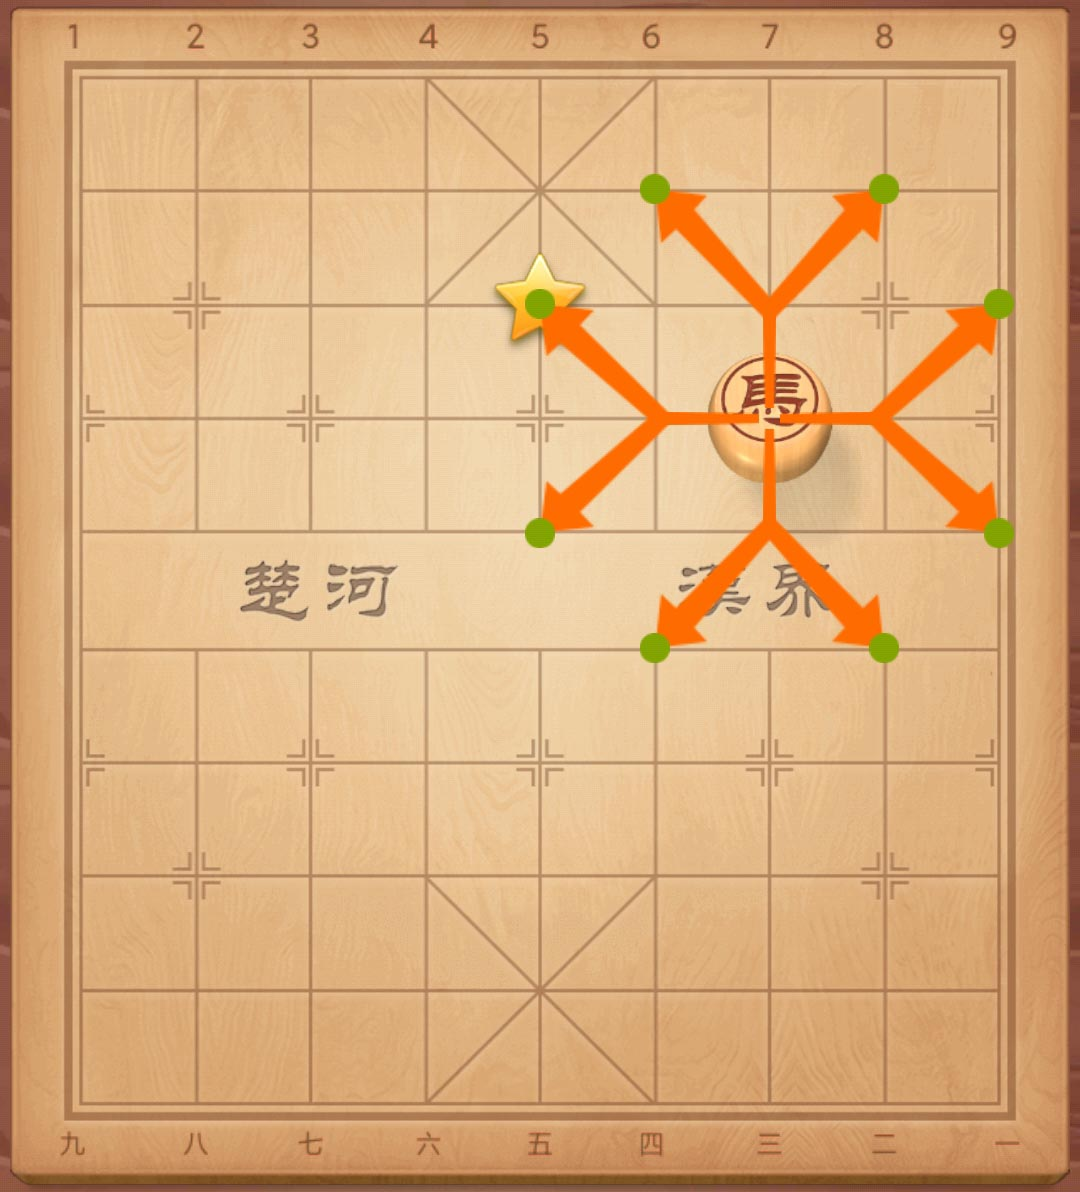
\includegraphics[scale=0.1]{images/chess.jpg}
\end{center}

\section*{输入格式}
一行,四个整数$x_1,y_1,x_2,y_2(1 \leq x_1,x_2 \leq 10; 1 \leq y_1,y_2 \leq 9)$

\section*{输出格式}
一行,一个整数:若马能从$p1$走到$p2$,输出马从$p1$走到$p2$最少需要多少步;否则输出-1。

\section*{输入输出样例}
\begin{tabularx}{450pt}{X|X}
	\toprule
	输入样例 & 输出样例 \\
	\midrule
	1 1 2 3  & 1        \\
	\bottomrule
\end{tabularx}
\vspace{0.5cm}

\begin{tabularx}{450pt}{X|X}
	\toprule
	输入样例 & 输出样例 \\
	\midrule
	5 5 5 5  & 0        \\
	\bottomrule
\end{tabularx}
\vspace{0.5cm}

\begin{tabularx}{450pt}{X|X}
	\toprule
	输入样例 & 输出样例 \\
	\midrule
	8 5 10 8 & 3        \\
	\bottomrule
\end{tabularx}

\newpage
\chapter*{C.\quad \ref*{pro:3}}
\begin{center}
	运行时间上限:\ref*{tim:3} \quad 运行内存上限:\ref*{mem:3} \quad 题目类型:\ref*{typ:3} \quad 命题人:\ref*{aut:3}
\end{center}

\section*{题目描述}
双端队列是一种常用的数据结构,其支持四种操作:在队头插入一个元素、在队尾插入一个元素、弹出队头的元素、弹出队尾的元素。(弹出:即将元素从双端队列中拿走)

给你一个存放有$1 \sim n$的\textbf{一个排列}的双端队列,你可以对其进行若干次弹出操作(可以弹出队头或队尾),且弹出的元素按弹出顺序排列出的数列必须为递增的,请问最多可以弹出多少个元素?

例如:如下双端队列最多可以弹出$4$个元素,操作顺序为弹出队首元素$2$、弹出队尾元素$3$、弹出队尾元素$4$、弹出队尾元素$5$。

\begin{center}
	\begin{tabularx}{200pt}{M|M|M|M|M}
		\toprule
		2 & 1 & 5 & 4 & 3 \\
		\bottomrule
	\end{tabularx}
\end{center}

\section*{输入格式}
第一行,一个整数,$n(1 \leq n \leq 5 \times 10^5)$。

第二行,$n$个整数,代表初始的双端队列。

\section*{输出格式}
一行,一个整数:最多能取出多少个数字。

\section*{输入输出样例}
\begin{tabularx}{450pt}{X|X}
	\toprule
	输入样例  & 输出样例 \\
	\midrule
	5         & 4        \\
	2 1 5 4 3 &          \\
	\bottomrule
\end{tabularx}
\vspace{0.5cm}

\begin{tabularx}{450pt}{X|X}
	\toprule
	输入样例      & 输出样例 \\
	\midrule
	7             & 7        \\
	1 3 5 6 7 4 2 &          \\
	\bottomrule
\end{tabularx}
\vspace{0.5cm}

\begin{tabularx}{450pt}{X|X}
	\toprule
	输入样例 & 输出样例 \\
	\midrule
	3        & 3        \\
	1 2 3    &          \\
	\bottomrule
\end{tabularx}
\vspace{0.5cm}

\begin{tabularx}{450pt}{X|X}
	\toprule
	输入样例 & 输出样例 \\
	\midrule
	4        & 4        \\
	1 2 4 3  &          \\
	\bottomrule
\end{tabularx}

\newpage
\chapter*{D.\quad  \ref*{pro:4}}
\begin{center}
	运行时间上限:\ref*{tim:4} \quad 运行内存上限:\ref*{mem:4} \quad 题目类型:\ref*{typ:4} \quad 命题人:\ref*{aut:4}
\end{center}

\section*{题目描述}
有$n$个矿泉水瓶,第$i$个瓶子里装有$a_i\ ml$水。

AgOH会对你进行$m$次询问,每次询问一个区间$[l,r]$,请你告诉AgOH第$l$个瓶子到第$r$瓶子之间(包含第$l$个和第$r$个)的所有瓶子里共装有多少$ml$的水。

\section*{输入格式}
第一行,两个整数$n,m(1 \leq n,m \leq 10^6)$。

第二行,$n$个整数$a_i(1 \leq a_i \leq 550)$。

第三到第$m+1$行:每行两个整数$l,r(1 \leq l \leq r \leq 10^6)$。

\section*{输出格式}
共$m$行,第$i$行代表第$i$次询问的答案。

\section*{输入输出样例}
\begin{tabularx}{450pt}{X|X}
	\toprule
	输入样例  & 输出样例 \\
	\midrule
	5 3       & 3        \\
	1 2 3 4 5 & 9        \\
	1 2       & 15       \\
	2 4       &          \\
	1 5       &          \\
	\bottomrule
\end{tabularx}

\newpage
\chapter*{E.\quad \ref*{pro:5}}
\begin{center}
	运行时间上限:\ref*{tim:5} \quad 运行内存上限:\ref*{mem:5} \quad 题目类型:\ref*{typ:5} \quad 命题人:\ref*{aut:5}
\end{center}

\section*{题目描述}
本次比赛实验室内座位布局方式参考……打麻将。

既然都坐成了棋牌室的样子了,不打打麻将实在是说不过去。

当然比赛过程中打一局完整的麻将是不现实的,你只需要判断一副手牌是否是和牌即可。

\begin{remark}
	\hspace{0.15cm} \textbf{和牌规则}:对于手中的14张手牌,和牌需达成以下条件:

	\begin{itemize}
		\item 有一个 \textbf{雀头}。
		\item 有四个 \textbf{面子}。
		\item 雀头和各个面子间没有交叉的牌
	\end{itemize}

	\hspace{0.15cm} \textbf{雀头}:两张同花色的牌,如 
\includegraphics[scale=0.5]{images/mahjong/1s.png} 
\includegraphics[scale=0.5]{images/mahjong/1s.png}

	\hspace{0.15cm} \textbf{面子}:包括 \textbf{刻子} 和 \textbf{顺子} (不要问为啥没杠,莫抬杠)

	\begin{itemize}
		\item \textbf{刻子}:三张同花色的牌,如 
\includegraphics[scale=0.5]{images/mahjong/1m.png} 
\includegraphics[scale=0.5]{images/mahjong/1m.png} 
\includegraphics[scale=0.5]{images/mahjong/1m.png}。
		\item \textbf{顺子}:三张相邻的同类型牌(只包括条/索、饼/筒、万三种),如 
\includegraphics[scale=0.5]{images/mahjong/1m.png} 
\includegraphics[scale=0.5]{images/mahjong/2m.png} 
\includegraphics[scale=0.5]{images/mahjong/3m.png}。
\includegraphics[scale=0.5]{images/mahjong/9m.png} 与
\includegraphics[scale=0.5]{images/mahjong/1m.png}、
\includegraphics[scale=0.5]{images/mahjong/9p.png} 与
\includegraphics[scale=0.5]{images/mahjong/1p.png}、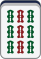
\includegraphics[scale=0.5]{images/mahjong/9s.png} 与
\includegraphics[scale=0.5]{images/mahjong/1s.png} 不算作相邻
	\end{itemize}

\end{remark}


\section*{输入格式}
第一行,一个整数$t$,代表共有$t$组数据。

第$2 \sim t+1$行,每行$14$个用空格分隔开的双字符字符串,代表一副手牌。手牌表示规则如下:

\begin{itemize}
	\item 一个$1 \sim 9$的数字$x+$一个小写字母$b$,代表$x$饼(也叫$x$筒)。例如$2b$代表 
\includegraphics[scale=0.5]{images/mahjong/2p.png}。
	\item 一个$1 \sim 9$的数字$x+$一个小写字母$t$,代表$x$条(也叫$x$索)。例如$8t$代表 
\includegraphics[scale=0.5]{images/mahjong/8s.png}。
	\item 一个$1 \sim 9$的数字$x+$一个小写字母$w$,代表$x$万。例如$5w$代表 
\includegraphics[scale=0.5]{images/mahjong/5m.png}。
	\item 一个$1 \sim 7$的数字$x+$一个小写字母$z$,从$1z \sim 7z$分别代表 
\includegraphics[scale=0.5]{images/mahjong/1z.png}、
\includegraphics[scale=0.5]{images/mahjong/2z.png}、
\includegraphics[scale=0.5]{images/mahjong/3z.png}、
\includegraphics[scale=0.5]{images/mahjong/4z.png}、
\includegraphics[scale=0.5]{images/mahjong/5z.png}、
\includegraphics[scale=0.5]{images/mahjong/6z.png}、
\includegraphics[scale=0.5]{images/mahjong/7z.png}。
\end{itemize}

数据保证只会出现以上样式的牌。与正常的一副麻将不同,每张牌的出现次数\textbf{不限},例如可能出现14张白的情况,且这种情况是和牌。

\section*{输出格式}
共$t$行,第$i$行代表第$i$组数据的答案:若该组牌为和牌,输出\lstinline{Tsumo!};反之输出\lstinline{Waiting for Tsumo!}

\section*{输入输出样例}
\begin{tabularx}{450pt}{X|X}
	\toprule
	输入样例 & 输出样例 \\
	\midrule

	\bottomrule
\end{tabularx}

\newpage
\chapter*{F.\quad \ref*{pro:6}}
\begin{center}
	运行时间上限:\ref*{tim:6} \quad 运行内存上限:\ref*{mem:6} \quad 题目类型:\ref*{typ:6} \quad 命题人:\ref*{aut:6}
\end{center}

\section*{题目描述}
游戏《明日方舟》里,干员异客的攻击方式为:攻击造成\textbf{法术伤害},且会在$4$个敌人间跳跃,每次跳跃伤害降低$15\%$并造成短暂停顿。

法术伤害会受到敌人\textbf{法抗}的百分比削减,即若对一个\textbf{法抗}为$p\%$的敌人造成$s$点\textbf{法术伤害},该敌人仅会受到$s \times (1-p\%)$点\textbf{真实伤害}。

假设敌人具有无限点血量,给出异客的攻击力和四个被击中的敌人的法抗,请你计算出异客一次攻击造成了多少伤害。

注意:因为敌人的血量为整数,所以对\textbf{每个敌人}打出的\textbf{真实伤害}都需要向下取整。

\section*{输入格式}
第一行,一个整数$t$,代表共有$t$组数据。

第$2 \sim t+1$行,每行$5$个整数,分别代表异客的攻击力$A(1 \leq A \leq 1500)$和依次被击中的$4$个敌人的法抗$k_1,k_2,k_3,k_4(0 \leq k_i \leq 100)$

\section*{输出格式}
共$t$行,第$i$行代表第$i$组数据的答案

\section*{输入输出样例}
\begin{tabularx}{450pt}{X|X}
	\toprule
	输入样例 & 输出样例 \\
	\midrule

	\bottomrule
\end{tabularx}

\end{document}